\begin{mainquestion}{resistor_search}{Current Source Design}

\questionpoints Consider a \SI{110}{\milli\ampere} current source with source resistance $R_{s}$ connected to a load $R_{L}$ as shown in the attached figure. You wish to find single, standard resistance values (\SI{1}{\ohm} or higher) (assume \href{https://asenergi.com/pdf/resistors/standard-resistor-values-e24.pdf}{E24 series} also in Hambley Table B.1) for each resistor such that the current through the load is as close to \SI{17}{\milli\ampere} as possible, while minimizing the overall power dissipated in the circuit.

\begin{center}
    % [width=0.8\textwidth] makes the image take up 80% of the text width
    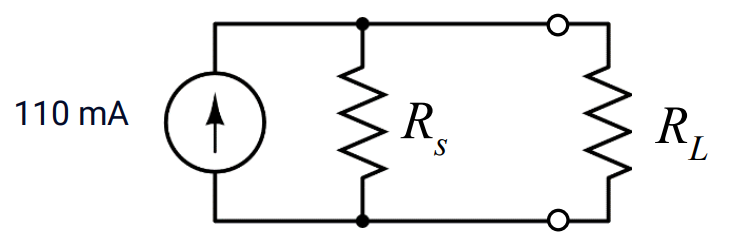
\includegraphics[width=0.5\textwidth]{current_source.png}
\end{center}

% =========================================================
\begin{partquestion}{findvalue}
{Find the values for $R_{s}$ and $R_{L}$ that satisfy these constraints, assuming the resistors accurately match their marked values.}

\begin{answer}[3in]
\end{answer}

\end{partquestion}

% =========================================================
\begin{partquestion}{deviation}
{Calculate the \% deviation from the desired load current.}

\begin{answer}[1.5in]
\end{answer}

\end{partquestion}

% =========================================================
\begin{partquestion}{power}
{Calculate the total power dissipated in the circuit.}

\begin{answer}[1.5in]
\end{answer}

\end{partquestion}

\end{mainquestion}
